\documentclass[a4paper]{article}

\usepackage[portuges,english]{babel}
\usepackage[latin1]{inputenc}
\usepackage{fancyvrb}
\usepackage{graphicx}
\usepackage[a4paper,left=20mm,right=20mm,bottom=20mm,top=15mm]{geometry}
\usepackage{moreverb}
\usepackage{amsthm}
\usepackage{listings}
\usepackage{indentfirst}
\usepackage{hyperref}

\lstset{
	language=C,
	basicstyle=\scriptsize\sffamily,
	numbers=left,
	stepnumber=1,
	numberstyle=\tiny, 
	showtabs=false,
	tabsize=1,
	breaklines=true,
	morecomment=[l]{//},
	xleftmargin=10mm,
	xrightmargin=10mm
	}

\hypersetup{colorlinks,
            citecolor=black,
            filecolor=black,
            linkcolor=black,
            urlcolor=black,
            pdftex}


\title{Precomputing Avatar Behaviour From Human Motion Data}

\date{\today}

\newtheorem{constr}{CONSTRAINT}

\author{
Nuno A. Silva\\ \small pg17455@alunos.uminho.pt \\ Universidade do Minho
\and
Luis Miranda\\ \small pg14439@alunos.uminho.pt \\ Universidade do Minho
}

\begin{document}

\maketitle

%\abstract


%%%%%%%%%%%%%%%%%%%%%%%%%%
\section{Introduction}
%%%%%%%%%%%%%%%%%%%%%%%%%%
This report refers to a work based on a paper from Lucas Kovar, et. al\cite{motiongraphs}, particularly the path synthesis technique described there. Motion Graphs is a method for creating realistic, controllable motion. In Kovar's work a directed graph is automatically generated, this graph contains pieces of original motion and automatically generated transitions. The authors also presented a general framework for extracting a particular graph walk that meet the user's specifications, and apply this framework to a specific problem with different styles of locomotion and arbitrary paths. \\

Path synthesis relates to this final step in the proposed framework, where a user specifies a path and a graph walk is performed in order to generate the locomotion that best suits the path. The goal is to integrate this specific module into a larger virtual character locomotion system. Ideally the user defined path should be aproximated by a spline and then a search in the motion graph should be done in order to find a set of motion capture data that minimizes the error. This error is the sum of the squared differences between the defined path and the path that the animation will produce, for that it is used the arc-length distance of the paths. \\

The OGRE engine will be used as the basis for the entire project. A scene with a model is generated where the user can input the desired path to traverse. Once the program finds the set of motions that respect the rules explained above, it is rendered on the scene. \\



%%%%%%%%%%%%%%%%%%%%%%%%%%
\section{Implementation details}
%%%%%%%%%%%%%%%%%%%%%%%%%%
The implementation can be divided in three  different parts, step one, where the user define the path, step two, were the animations are chosen and step three, where the animation that follows the user path is shown. Each one is a fundamental operation of the whole system. The whole process is depicted in the workflow on figure ~\ref{fig:work}, it entirely coded into \texttt{frameRenderingQueued} method of Ogre engine, other methods like \texttt{createScene}, \texttt{keyPressed} or \texttt{mousePressed} do, respectively, the scene setup, variables and structures initializations and path definition. \\


\begin{figure}[hbtp]
\begin{center}
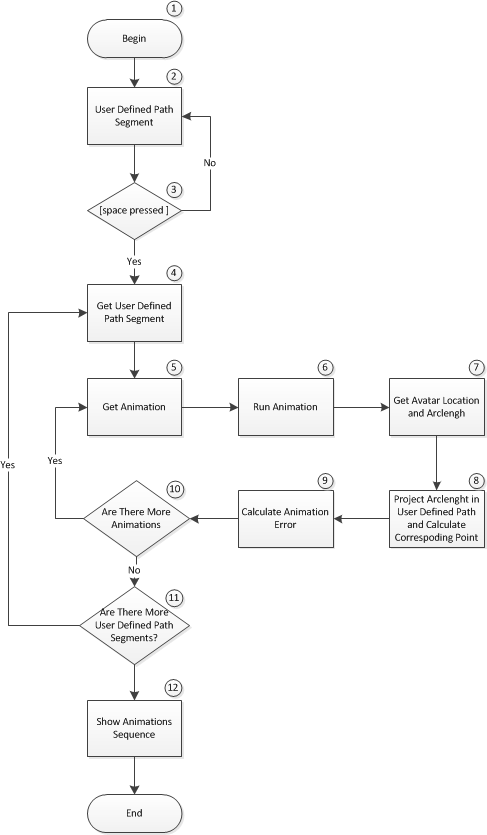
\includegraphics[scale=0.8]{Images/fluxograma.png} 
\caption{\textit{Workflow}}
\label{fig:work}
\end{center}
\end{figure}



%	USERPATH DEFINITION
\subsection{Path definition}
User path definition (step 1 in picture ~\ref{fig:work}) is the step where the user defines a simple path which the avatar would ideally travel.   The user defined path is a sequence of vectors between points chosen by the user in the application screen (picture ~\ref{fig:uapath}). The user, using the mouse, can define a set of points in a plane. This points will be used in the construction of a line that passes trough them. Ideally this line should be a spline (picture ~\ref{fig:uapath}), but in the current state, our work only supports a straight path between each pair of points. \\

\begin{figure}[hbtp]
\begin{center}
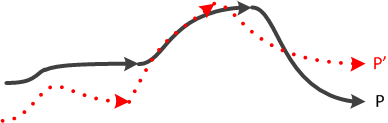
\includegraphics[scale=0.8]{Images/UserPathVSAvatarPath.png} 
\caption{\textit{User defined path(bold line) and avatar path(dot line)}}
\label{fig:uapath}
\end{center}
\end{figure}

In picture ~\ref{fig:uapath}, one can see as an example, in bold, the user defined path, and in dots a path that the avatar could effectively follow.  \\





%	ERROR EVALUATION
\subsection{Error Evaluation}
After the path is defined, the user can press the space key (step 3 in picture ~\ref{fig:work}), so that the next phase, where the animations are evaluated for error, starts. \\

To make an animation that runs along the path defined by the user, a set of animations from motion capture data must be chosen.  However, not all animations are suitable for a path defined by the user. This arises the question, how to choose animations that fit the path defined by the user? The answer to this question is to associate to each animation, an error. This error will depend of the path followed by the animation, and it will be greater if the animation deviates largely from the user defined path and smaller, if the animation, follows a path that is similar to the one defined by the user.  \\

\begin{figure}[hbtp]
\begin{center}
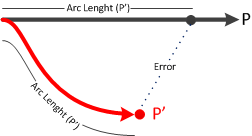
\includegraphics[scale=0.8]{Images/error.png} 
\caption{\textit{Error definition}}
\label{fig:error}
\end{center}
\end{figure}

Let $P$ be the user defined path, and $P'$ the path the avatar made (by projecting the root bone onto de floor). First a segment from the path $P$ defined by the user is selected. For this segment, before the error can be calculated, the software must load and display the animations, so the path travelled by each one of them can be measured. This operation is done following Ogre\textquoteright s method for displaying animations. To start, all the animations available for the current avatar are loaded. Then, for each one of these animations, we start by running it ($P'$ on figure ~\ref{fig:error}). After the animation reaches the end, we can start calculating the error (steps 8, 9 and 9 in figure ~\ref{fig:error}). The error can be defined as the arclength distance of the point where the animation ends, in the animation path ($P'$) and the point at the same arclength in the user defined path ($P$).  \\

We start by projecting the arclength of $P'$ in $P$, so we can discover the point in $P$ that corresponds to the point with the same arclength as the endpoint in $P'$. The arclength can either be smaller than the path $P$ or greater than the path $P$.
%If the arclength is smaller, one can simply calculate the point recurring to the parametric equation of a line in 3D space\footnote{}.  If the arclength is greater than the length of $P$, the error is calculated using the end point of $P$. \\
We calculate it by summing the magnitude of the segments of $P$ until it equals the arclength of $P'$. The arclenght of $P'$ is estimated by summing the root bone translations at each frame. \\

We then choose and save the animation with the smallest error, which is the one that will, most closely, follow a path similar to the one defined by the user. The process is repeated for all animations for each segment of the user defined path. \\






%	SHOW THE CALCULATED MOTION PATH
\subsection{Calculated motion path}

When all the segments of the defined path have been traversed, the animations in the calculated motion path are shown. In OGRE, the position of the node holding the avatar entity must be updated at the end of its animation. 






%%%%%%%%%%%%%%%%%%%%%%%%%%
\section{Conclusion and future work}
%%%%%%%%%%%%%%%%%%%%%%%%%%

Thought this project, we encountered some non expected problems:
\begin{itemize}
	\item Atop not being acquainted to programming in OGRE, our initial approach used some example animated models included in OGRE, while we waited for the final data structures from the other groups. This initial approach was all wrong as the models did not correspond at all to what we would be dealing with.
	\item When we got some animations from our motion capture sessions, but still without the full specification of other groups, we were forced to use OGRE's data structures and API, \texttt{AnimationState}, which do not expose the could points. Due to this we had to explictly render each frame of the animation in order to discover its positions.
\end{itemize}


The implementation can still improve in many ways. For a start, the correct display of the calculated motion path. Also splines should be used for the user defined path. Aditionally, it would be good to improve the user interaction with the program, and finally fully integrate it with the remaining system.





%%%%%%%%%%%%%%%%%%%%%%%%%%
\begin{thebibliography}{}

\bibitem{motiongraphs}
{Lucas Kovar, Michael Gleicher and Frederic Pighin},{Motion Graphs}, {2002}
    
    
\end{thebibliography} 


\end{document}
